\documentclass[11pt]{article}
\usepackage{geometry}
 \geometry{
 a4paper,
 total={170mm,257mm},
 left=20mm,
 top=20mm,
 }
%Gummi|065|=)
\title{\textbf{CS747 - Assignment 1}}
\author{Kalpesh Krishna\\140070017\\kalpeshk2011@gmail.com}
\date{}
\usepackage{graphicx}
\begin{document}

\maketitle

\section{Implementation}
All algorithms were implemented in C++ building upon the basecode provided. An initial class \texttt{BaseAlgorithm} has been created in \texttt{algorithm-data.h}. Each algorithm inherits from this class. The main implementations are located in \texttt{algorithm-data.cpp}.
\subsection{Epsilon Greedy}
Using \texttt{gsl\_rng\_uniform}, an initial Bernoulli distribution for $\epsilon$ is sampled. For the first pull, this choice is ignored and the system explores randomly. For the exploration step, \texttt{gsl\_rng\_uniform} has been used again. 10 values of $\epsilon \in \{0.1, 0.2, ... 1.0\}$ were tried, and the best value $\epsilon = 0.1$ was chosen. Further reduction of $\epsilon$ should reduce long term regret.
\subsection{UCB}
The UCB implementation exactly follows \textit{Auer et al. 2002} implementation with a initial round robin sampling round and subsequent maximization of the UCB objective.
\subsection{KL-UCB}
As outlined in the \textit{Garivier et al. 2011} paper, I've taken $c=0$. Taking $c=3$ resulted in worse long term regret. To approximate the value of $q$, a binary search in $q_a \in [\hat{p}_a, 1]$ (where KL-Divergence a strictly increasing function) was conducted. This search concluded when
\begin{center}
$0 \leq \frac{1}{N_a}(\log{T} + c\log{\log{T}}) - KL(\hat{p}_a, q) \leq 10^{-6}$
\end{center}
The threshold value and $c$ can be adjusted in \texttt{algorithm-data.h}
\subsection{Thompson Sampling}
The \texttt{gsl\_ran\_beta} function in the GSL was used to sample from the beta distribution.
\section{Results}
Each of the curves below consist of 37 horizon points.\\$h = \{10, 20, ... 90, 100, 200, ... 900, 1000, 2000, ... 9000, 10000, 20000, ... 90000, 100000 \}$. For each horizon point, 100 different random seeds were taken. The curves represent an average across these runs.\\
The results are consistent with the discussed theory. Since the \texttt{epsilon-greedy} algorithm has a linear regret, it's seen as an exponentially increasing function in a logarithmic scale. The other algorithms enjoy a roughly linear curve (logarithmic regret), with optimal results seen in the order, \texttt{Thompson-Sampling} $>$ \texttt{KL-UCB} $>$ \texttt{UCB} as we had initially expected. As expected, the regret is larger in the 25-arms case, since it's harder for the system to find the optimal arm.\\
It was surprising to see the zoomed in curve for a horizon upto 2000, with \texttt{UCB} and \texttt{KL-UCB} doing worse than \texttt{epsilon-greedy}, indicating larger constants with $O(\log(T))$ than $O(T)$. It was also surprising to see occasional dips in regret, which I later realized are possible stochastically.
\subsection{5 Arms}
\begin{center}
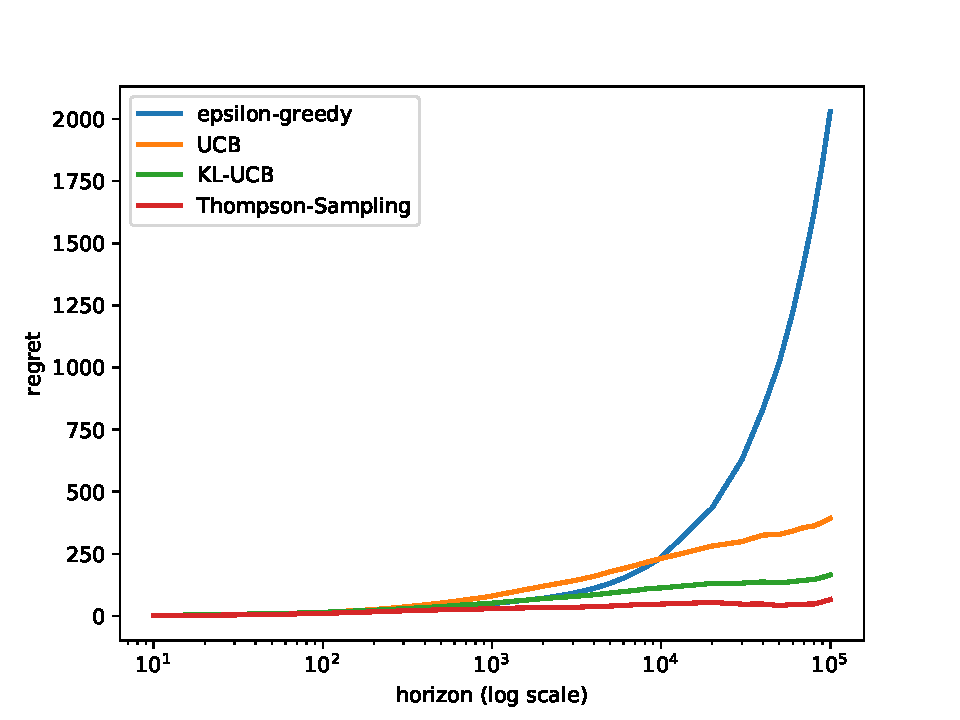
\includegraphics[width=15cm]{arms_5.pdf}
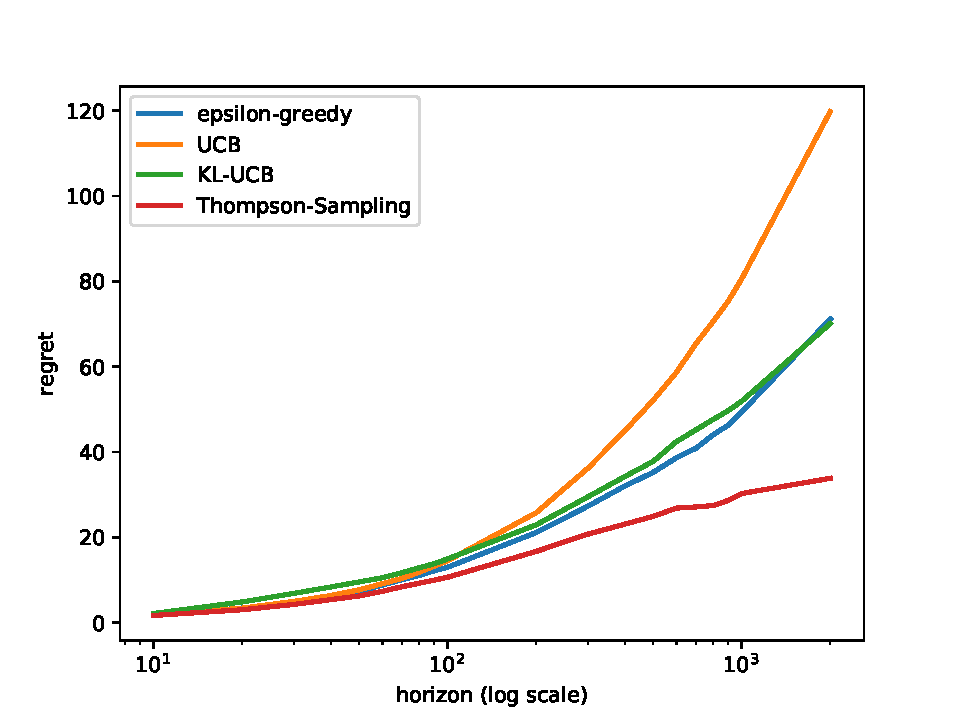
\includegraphics[width=15cm]{arms_5_zoom.pdf}
\end{center}
\subsection{25 Arms}
\begin{center}
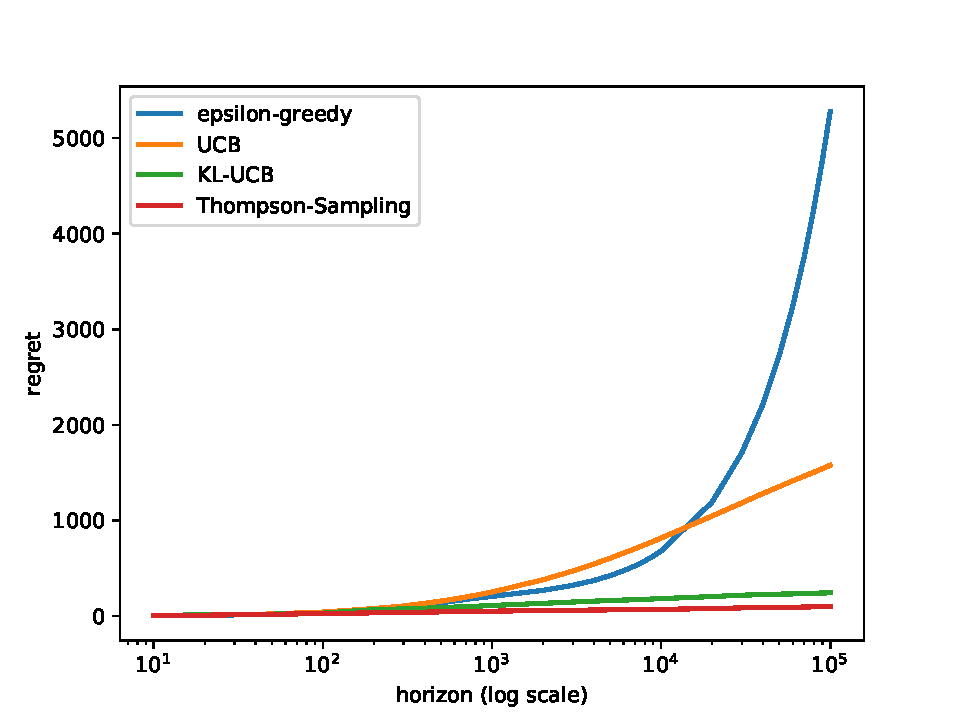
\includegraphics[width=15cm]{arms_25.pdf}
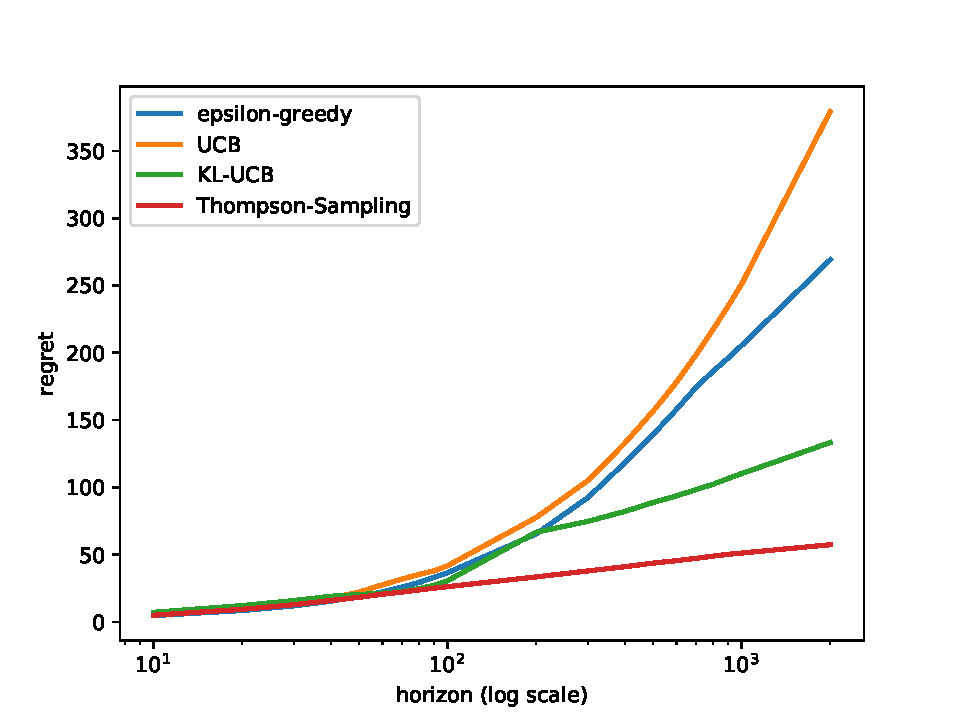
\includegraphics[width=15cm]{arms_25_zoom.pdf}
\end{center}
\end{document}
